% TITLE
\input{structure/title-page}
\input{helpers/empty-page}
\addtocounter{page}{-1}

% Declaration
\newpage
\chapter*{Declaration of Authorship}
\thispagestyle{empty}
% !TEX encoding = UTF-8 Unicode
\vspace*{1cm}

\large
\noindent
\IfLanguageName{ngerman}
{Ich versichere, dass ich die vorliegende Arbeit ohne fremde Hilfe und ohne Benutzung anderer als der angegebenen Quellen angefertigt \nobreak habe, und dass die Arbeit in gleicher oder \"ahnlicher Form noch keiner anderen Pr\"ufungsbeh\"orde vorgelegen hat und von dieser als Teil einer Pr\"ufungsleistung angenommen wurde. Alle Ausf\"uhrungen, die w\"ortlich oder sinngem\"a\s{} übernommen wurden, sind als solche gekennzeichnet.}
{I assure that I have produced the present work without the help of others and without using any sources other than those specified and that the work has not been submitted in the same or similar form to any other examination body and has been accepted as part of an examination. All statements, which have been taken literally or meaningfully, are marked as such.}
\vspace{3cm}

\begin{minipage}{0.45\textwidth}
	------------------------------------
	
	\IfLanguageName{ngerman}{Ort, Datum}{Location, Date}
	
\end{minipage}
\begin{minipage}{0.45\textwidth}
	------------------------------------
	
	\IfLanguageName{ngerman}{Unterschrift}{Signature}

	
\end{minipage}

\normalsize
\pagenumbering{Roman}
\input{helpers/empty-page}
\thispagestyle{empty}
\cleardoublepage

% Table of Contents
\addtocounter{page}{-2}
\setcounter{tocdepth}{1}
\tableofcontents
\clearpage


% Summary
\input{helpers/empty-page}
\chaptermark{Abstract}

\chapter*{Abstract}
\addcontentsline{toc}{chapter}{Abstract}
The task of acoustic source localisation and tracking has both a long history in the signal processing literature as well as many modern applications. In this thesis, the \glsentrylong{em} algorithm is utilised to solve this task, estimating the parameters of a \glsentrylong{gmm} which models the spatial information available from the received signals at an acoustical sensor array. Recursive variations of the algorithm for source localisation are presented to track moving speakers over time. Both Source Localisation and Tracking are tested in a simulation setup, where the algorithm's performance is evaluated in different scenarios. These evaluations show that localisation performance strongly depends on the conditions and is not reliable for highly reverberant and noisy environments with this method. Two versions of the source tracking algorithm, \glsentryshort{crem} and \glsentryshort{trem}, have been implemented and evaluated. These perform equally well across all evaluation scenarios. In general, these algorithms were able to track sources in mildly reverberant conditions. Also, high memory requirements and computational complexity are an issue for many practical applications.
\clearpage

% List of Abbreviations
\printglossary[type=\acronymtype, title=List of Abbreviations]
\clearpage

% List of Symbols
\renewcommand{\chaptermark}[1]{ \markboth{ \uppercase{#1}}{}}
\renewcommand{\sectionmark}[1]{ \markright{ \uppercase{#1}}{}}
\chaptermark{List of Symbols}
\sectionmark{List of Symbols}
%\renewcommand{\chaptermark}[1]{\markboth{\uppercase{\chaptername \ \thechapter.\ #1}}{}}
%\renewcommand{\sectionmark}[1]{ \markright{ \uppercase{\thesection.\ #1}}{}}

\chapter*{List of Symbols}
\addcontentsline{toc}{chapter}{List of Symbols}
\chaptermark{List of Symbols}
\sectionmark{List of Symbols}
\chapter*{List of Symbols}
\addcontentsline{toc}{chapter}{List of Symbols}

\subsubsection*{Notational Remarks}
The following notational conventions are followed throughout this thesis: A lower case regular letter indicates scalars, a lower case bold letter indicates vectors, and a capital bold letter indicates matrices.

%Positions in the cartesian coordinate system are described by their location vector $\bm p_{\text{index}}=[x, y, z]$ and are used for receiver locations $\bm p_m^i$ and source locations $\bm p_s$. The set of all possible positions is described by $\pall$.

%Sources are addressed by their index $s=1,\dots,S$ and receivers are addressed by their receiver pair $m\in[1, \dots, M]$ and pair index $i\in[1, 2]$. A braced superscript $l$, like $\psi^{(l)}$, denotes the iteration the \gls{em} algorithm is currently in, so $\psi^{(l-1)}$ indicates the value of $\psi$ of the preceding iteration. As recursions will be iterated with respects to the time-index, superscript $(t)$ (e.g. $\psi^{(t)}$) is used respectively. 
The diag$(\cdot)$ operator describes a diagonal matrix, where the elements in braces are placed on the diagonal, whereas all other entries of the matrix are equal to 0.


%% DEFINITIONS %%

% Single Symbols
\newcommand{\prp}{\bm\phi}

\newcommand{\p}{\bm p}
\newcommand{\ps}{\p_s}
\newcommand{\pr}{\p_m^i}
\newcommand{\pall}{\mathcal{P}}
\newcommand{\pinp}{\p \in \pall}

\newcommand{\psip}{\bm\psi_{\bm p}}
\newcommand{\psiRlast}{\bm\psi_R^{(t-1)}}
\newcommand{\psiRPlast}{\psi_{\bm p,R}^{(t-1)}}
\newcommand{\psiRnow}{\bm\psi_R^{(t)}}
\newcommand{\psiRPnow}{\psi_{\bm p,R}^{(t)}}
\newcommand{\psips}{\psi_{\bm p,s}}

% Functions
\newcommand{\gaussian}[1]{\mathcal{N}\left (#1\right )}
\newcommand{\pdffunc}{\psi_{\bm p}^{(l-1)}\prod_{m}\mathcal{N}^c\left (\phi^k_m(t,k);\tilde\phi^k_m(\bm p),\sigma^{2,(l-1)}\right )}
\newcommand{\pdffuncR}{\psi_{\bm p,R}^{(t-1)}\prod_{m}\mathcal{N}^c\left (\phi^k_m(t,k);\tilde\phi^k_m(\bm p),\sigma_R^{2,(t-1)}\right )}
\newcommand{\gauss}{\mathcal{N}^c\big(\phi_m(t,k);\tilde\phi^k_m,\sigma^2\big)}
\newcommand{\Q}{\mathcal{Q}\left (\theta\vert\theta^{(l-1)}\right )}
\newcommand{\mulast}{h^{(l)}(t,k,\bm p)}
\newcommand{\muRlast}{h(t,k,\bm p)}
\newcommand{\z}{z(t,k,\bm p)}
\newcommand{\lcompl}{\prod_{t,k}\sum_{\vect{p}}\psip\cdot\z\prod_{m}\gauss}

% Other
\newcommand{\vect}[1]{\mathbf{#1}}
\newcommand{\norm}[1]{|{#1}|_2}
\newcommand{\abs}[1]{|{#1}|_1}
\newcommand{\Tsixty}{T$_{60}$\ }

%% TABLE %%

\begin{longtable*}[l]{ll}
	\multicolumn{2}{l}{\textbf{Mathematical Operators}} \\[2pt]
	$|\cdot |$    & Absolute value (when applied to scalar)\\
	$|\cdot |$    & Cardinality (when applied to set)\\
	$\|\cdot \|$  & Length of vector (when applied to vector)\\
	$\|\cdot \|$  & Eucledian distance (when applied to difference of two vectors)\\
	det$(\cdot)$  & Determinant of matrix\\
	diag$(\cdot)$ & Diagonal matrix of vector\\

	\multicolumn{2}{l}{\textbf{Indices}} \\[2pt]
	$t$         & Time-bin index \\
	$k$         & Frequency-bin index \\
	$i$         & Receiver index \\
	$m$         & Sensor node index \\
	$s$         & Source index \\
	$l$         & Algorithm iteration index \\[6pt]

	\multicolumn{2}{l}{\textbf{Scalars}} \\[2pt]
	$T$         & Number of time-bins \\
	$K$         & Number of frequency-bins \\
	$M$         & Number of sensor nodes \\
	$S$         & Number of sources \\
	$L$         & Number of Iterations \\[6pt]

    \multicolumn{2}{l}{\textbf{Vectors}} \\[2pt]
	$\p $      & Location vector of grid point\\
	$\pall $      & Set of all grid points $\p$\\
	$\ps $      & Location vector of source $s$ \\
	$\pr $      & Location vector of receiver $i$ of sensor node $m$ \\

	$\prp$      & Vector of pair-wise relative phase ratios \\
	$\prp_m$      & Pair-wise relative phase ratio at sensor node $m$ \\
	$\psi$      & Weight of Gaussian mixture component \\
	$\psip$      & Vector of weights of Gaussian mixture components \\
\end{longtable*}

\clearpage
%\input{helpers/empty-page}


%%%%%%%%%%%%%%%%%%%  Main Text  %%%%%%%%%%%%%%%%%%%

% Formula Margins
\setlength{\belowdisplayskip}{0.5cm}
\setlength{\belowdisplayshortskip}{0.5cm}
\pagenumbering{arabic}

\renewcommand{\sectionmark}[1]{ \markright{ \uppercase{\chaptername \ \thechapter.\ #1}}{}}

\chapter{Introduction}
Here comes the introduction...
\section{Application scenarios}
Examples for possible applications of audio source localisation and tracking are teleconferencing, automated multimedia capture, smart meeting rooms, lecture theatres \cite{Lehmann2007}
\section{Overview of Existing Literature}
\section{Research Problem}
\section{Setting Constraints}
\begin{itemize}
	\item Number of speakers a-priori known
	\item ?
\end{itemize}
\section{Structure of Thesis}
	In the beginning, chapter \ref{chap:theory} will introduce the theoretical concepts, that the algorithms for location estimation and tracking reviewed in this thesis are based upon. Chapter \ref{chap:algorithms} then will formally define these algorithms. In chapter \ref{chap:implementation} the implementation of these algorithms in \matlab is shown and test scenarios to evaluate these implementations are defined. All relevant code is included in \ref{sec:appCode}. The results of these tests are presented and discussed in chapter \ref{chap:results}. Finally, the findings of this thesis are summarized in chapter \ref{chap:concl} and a conclusion towards the applicability of these findings to the general performance of the reviewed algorithms is drawn.
\section{Notation}
\newcommand{\vect}[1]{\mathbf{#1}}
For easier understanding of the mathematical terms included within this thesis, the norms of mathematical notation are followed. A bold font indicates vectors ($\vect{p}$, $\vect{v}$, \dots).

\begin{itemize}
	\item vectors
	\item matrices
	\item ?
\end{itemize}


\renewcommand{\sectionmark}[1]{ \markright{ \uppercase{\thesection.\ #1}}{}}
\chapter{Theoretical Background}
In this section, the main theoretical concepts needed for audio source localisation and tracking, as it is implemented here, are laid out and put into context. First, the signal model is defined and it is shown, which features of the signal are exploited to estimate the location of it's origin. As we are simulating the received signal, instead of using recordings, the approach used for simulating a received signal, that is influenced by room acoustics and noise, is shown and it's limitations are discussed. Next, the \newacronym{gmm}{GMM}{Gaussian Mixture Model} \gls{gmm} is introduced as a mathematical representation of the possible locations of the audio sources, that are to be estimated. Last, the \newacronym{em}{EM}{Expectation-Maximization} \gls{em} Algorithm is explained and it is shown, how it can be used to estimate and optimise the parameters of the \gls{gmm} to yield the most likely source locations.

\section{Signal Model}
\label{sec:signal}
Received signal:
\begin{equation}
	z_m^i(t,k)=\sum_{s=1}^{S}a_{sm}^i(t,k)\cdot v_s(t,k)+n_m^i(t,k)
\end{equation}
Acoustic transfer function:
\begin{equation}
	a_{sm}^i(t,k)\approx\frac{1}{\|\mathbf{p}_s-\mathbf{p}_m^i\|}\cdot\exp{\left(-j\frac{2\pi k}{K}\frac{\tau^i_{sm}}{T_s}\right)}
\end{equation}
Signal travel time:
\begin{equation}
	\tau^i_{sm}=\frac{1}{c}\cdot\left(\|\mathbf{p}_s-\mathbf{p}_m^i\|\right)
\end{equation}

\section{Simulation of Room Acoustics}
\label{sec:simulation}
To simulate the setup described in \ref{sec:setup}, the image method for simulating small-room acoustics is used \cite{Allen1979}.

\section{\acrfull{gmm}}
\label{sec:gmm}
\begin{equation}
	\phi(t,k)\sim\sum_{s,\mathbf{p}}\psi_{s\mathbf{p}}\cdot\big(\phi(t,k);\tilde\phi^k(\mathbf{p}),\Sigma_s\big)
\end{equation}

\section{EM-Algorithm}
\label{sec:em}
The \acrfull{em} algorithm is an important algorithm in probabilistic theory \cite{Schwartz2014}.
\chapter{Description of algorithms}
\label{chap:algorithms}


\section{Location estimation}
\label{sec:algLocEst}

\section{Source Tracking}
\label{sec:algSrcTrack}

\newacronym{rem}{REM}{Recursive \acrfull{em}}
\newacronym{crem}{CREM}{\citeauthor{Cappe2009}'s Recursive Expectation-Maximisation}
\newacronym{trem}{TREM}{\citeauthor{Titterington1984}'s Recursive Expectation-Maximisation}

To integrate data from prior steps into each \gls{em} iteration, recursive variations of the \gls{em} algorithm have been developed. These will be called \gls{rem} algorithms in the upcoming sections.

In \cite{Schwartz2014}, two different \gls{rem} algorithms for speaker tracking are proposed. The first one is based on \citeauthor{Cappe2009}'s \gls{rem} and will be referenced as \acrshort{crem}, whereas the second one is based on \citeauthor{Titterington1984}'s \gls{rem} algorithm and will be called \acrshort{trem}.

\subsection{CREM algorithm}
\label{sec:crem}
\import{equations/}{alg-crem}

\subsection{TREM algorithm}
\label{sec:trem}
\import{equations/}{alg-trem}

\chapter{Implementation Details}
\label{chap:implementation}
Before any results can be produced, the described algorithms and setup have to be implemented and tested within a simulation framework, that allows for easy parameter customisation and evaluation. Therefore, what follows is the description of the different parts of the implementation that allows for the evaluation of the algorithms described in \ref{chap:algorithms}. First, the setup is defined and the simulation framework is laid out. Then, the implementation of both source localisation and source tracking are discussed. Lastly, evaluation scenarios are established to analyse the possibilities and limitations of the implementation. This will assist in drawing conclusions about the strengths and shortcomings of the algorithm in this particular setup and may allow for more general findings to be deducted.

\begin{figure}[H]
	\centering
	\begin{tikzpicture}
  \tikzset{
    block/.style={
      draw,
      minimum height=1cm,
      inner sep=1em,
    },
    arrow/.style={thick, ->, >=stealth}
    }
  \begin{scope}[start chain=transition going right,node distance=1cm]
    \node (sim)[block,on chain, minimum width=2cm] {simulate};
    \node (stft)[block,on chain, minimum width=2cm] {stft};
    \node (em)[block,on chain,minimum width=2cm] {em-algorithm};
    \node (loc)[block,on chain,minimum width=2cm] {estimate location};
    
    \draw [arrow] (sim) -- node[anchor=west] {} (stft);
    \draw [arrow] (stft) -- node[anchor=west] {} (em);
    \draw [arrow] (em) -- node[anchor=west] {} (loc);
  \end{scope}
\end{tikzpicture}
	\caption{Block diagram of execution steps}
	\label{diag:execBlocks}
\end{figure}


\section{Setup}
\label{sec:setup}
\import{chapters/4.implementation/}{setup}

\section{Simulation framework}
\newglossaryentry{RIR}
{
  name={RIR},
  description={room impulse response},
  first={\glsentrydesc{RIR} (\glsentrytext{RIR})},
  plural={RIRs},
  descriptionplural={room impulse responses},
  firstplural={\glsentrydescplural{RIR} (\glsentryplural{RIR})}
} 

\paragraph{Simulation of RIRs}
For the simulation of the \glspl{RIR} for the static location estimation case, the \emph{RIR-Generator} by \citeauthor{Habets2014} is used \cite{Habets2014}.

For the source trajectory simulation, execution time of the RIR-Generator increases drastically. Therefore, the \emph{fastISM} package by \citeauthor{Lehmann2010} is used \cite{Lehmann2010}.
\begin{figure}[H]
	\centering
	\tikzstyle{every node}=[draw=black,thick,anchor=west]
\tikzstyle{selected}=[draw=black,fill=yellow!20]
\tikzstyle{optional}=[dashed,fill=gray!50]
\begin{tikzpicture}[%
  grow via three points={one child at (0.5,-0.7) and
  two children at (0.5,-0.7) and (0.5,-1.4)},
  edge from parent path={(\tikzparentnode.south) |- (\tikzchildnode.west)}]
  \node [selected]{src} 
    child { node {config-update}}		
    child { node {simulate}}
    child { node {stft}}
    child { node {estimate-location}}
    child { node {estimation-error}}		
%    child { node {example}
%      child { node [selected] {generic}}
%      child { node [optional] {latex}}
%      child [missing] {}	
%      child { node {plain}}
%    }
;
\end{tikzpicture}
	\caption{Functions of Simulation Framework}
	\label{diag:simulationFramework}
\end{figure}

%\import{chapters/4.implementation/simulation-framework}

\section{Location estimation}
\section{Source tracking}
\section{Evaluation scenarios}
\chapter{Evaluation Results}
\label{chap:results}

\section{Location estimation}
\subsection*{Varying the number of sources}

\begin{figure}[H]
	\centering
	\begin{subfigure}{0.50\textwidth}
		\includestandalone[width=\textwidth]{data/plots/mean-err-n-sources}	
	\end{subfigure}
	\begin{subfigure}{0.35\textwidth}
		\includestandalone[width=\textwidth]{data/tables/mean-err-n-sources}	
	\end{subfigure}
%	\import{data/tables/}{mean-err-n-sources}
	\label{Mean localisation error across number of sources}
\end{figure}

\begin{figure}[H]
	\centering
	\import{data/plots/}{mean-err-n-sources-scatter}
	\label{Mean localisation error across number of sources}
\end{figure}

\begin{figure}[H]
	\centering
	\import{data/plots/}{mean-err-n-sources-box}
	\label{Mean localisation error across number of sources}
\end{figure}






\section{Source tracking}
\chapter{Conclusions}
\label{chap:concl}

\section{Critical review}
\section{Further research}


%\chapter[Testbed]{Testbed}
\chaptermark{Testbed}
\label{chap:Testbed}
This is a section, where LaTeX functionality can be tested!
\section{Graphics}
\subsection{Including .eps-files}

\begin{figure}[H]
\centering
\includegraphics[width=0.5\textwidth]{static/gaussian}
\caption{Multiple three-dimensional gaussian distributions...}
\label{fig:mog}
\end{figure}


This is the text beneath an included picture. Figure \ref{fig:mog} shows an example of how to include eps-figures in this document.

\subsection{Including tikz-figures}
Graphs can be included, like is shown in figure \ref{fig:sin}, using the input-method.
\tikzset{every picture/.style={scale=0.9}}
\begin{figure}[H]
	\centering
	% This file was created by matlab2tikz.
%
%The latest updates can be retrieved from
%  http://www.mathworks.com/matlabcentral/fileexchange/22022-matlab2tikz-matlab2tikz
%where you can also make suggestions and rate matlab2tikz.
%
\definecolor{mycolor1}{rgb}{0.00000,0.44700,0.74100}%
%
\begin{tikzpicture}

\begin{axis}[%
width=6.028in,
height=4.754in,
at={(1.011in,0.642in)},
scale only axis,
xmin=0,
xmax=6.28318530717959,
xtick={0,1.5707963267949,3.14159265358979,4.71238898038469,6.28318530717959},
xticklabels={{0},{$\text{1/2 }\pi$},{$\pi$},{$\text{3/2 }\pi$},{$\text{2}\pi$}},
ymin=-1.5,
ymax=1.5,
ytick={-1,  0,  1},
axis background/.style={fill=white}
]
\addplot [color=mycolor1, forget plot]
  table[row sep=crcr]{%
0	0\\
0.126933036508679	0.126592453573749\\
0.253866073017357	0.251147987181079\\
0.380799109526036	0.371662455660328\\
0.507732146034714	0.486196736100469\\
0.634665182543393	0.59290792905464\\
0.761598219052071	0.690079011482112\\
0.88853125556075	0.776146464291757\\
1.01546429206943	0.849725429949514\\
1.14239732857811	0.909631995354518\\
1.26933036508679	0.954902241444074\\
1.39626340159546	0.984807753012208\\
1.52319643810414	0.998867339183008\\
1.65012947461282	0.996854775951942\\
1.7770625111215	0.978802446214779\\
1.90399554763018	0.945000818714669\\
2.03092858413886	0.895993774291336\\
2.15786162064753	0.832569854634771\\
2.28479465715621	0.755749574354258\\
2.41172769366489	0.666769000516292\\
2.53866073017357	0.567059863862771\\
2.66559376668225	0.458226521727411\\
2.79252680319093	0.342020143325669\\
2.91945983969961	0.220310532786541\\
3.04639287620828	0.0950560433041829\\
3.17332591271696	-0.0317279334980679\\
3.30025894922564	-0.15800139597335\\
3.42719198573432	-0.281732556841429\\
3.554125022243	-0.400930535406613\\
3.68105805875168	-0.513677391573406\\
3.80799109526036	-0.618158986220605\\
3.93492413176903	-0.712694171378863\\
4.06185716827771	-0.795761840530832\\
4.18879020478639	-0.866025403784438\\
4.31572324129507	-0.922354294104581\\
4.44265627780375	-0.963842158559942\\
4.56958931431243	-0.989821441880933\\
4.69652235082111	-0.999874127673875\\
4.82345538732978	-0.993838464461254\\
4.95038842383846	-0.971811568323542\\
5.07732146034714	-0.934147860265107\\
5.20425449685582	-0.881453363447582\\
5.3311875333645	-0.814575952050336\\
5.45812056987318	-0.734591708657534\\
5.58505360638185	-0.64278760968654\\
5.71198664289053	-0.540640817455597\\
5.83891967939921	-0.429794912089172\\
5.96585271590789	-0.312033445698487\\
6.09278575241657	-0.189251244360411\\
6.21971878892525	-0.0634239196565654\\
6.34665182543393	0.0634239196565649\\
6.4735848619426	0.18925124436041\\
6.60051789845128	0.312033445698487\\
6.72745093495996	0.429794912089172\\
6.85438397146864	0.540640817455597\\
6.98131700797732	0.642787609686539\\
7.108250044486	0.734591708657533\\
7.23518308099467	0.814575952050335\\
7.36211611750335	0.881453363447582\\
7.48904915401203	0.934147860265107\\
7.61598219052071	0.971811568323542\\
7.74291522702939	0.993838464461254\\
7.86984826353807	0.999874127673875\\
7.99678130004675	0.989821441880933\\
8.12371433655542	0.963842158559942\\
8.2506473730641	0.922354294104582\\
8.37758040957278	0.866025403784439\\
8.50451344608146	0.795761840530832\\
8.63144648259014	0.712694171378863\\
8.75837951909882	0.618158986220606\\
8.88531255560749	0.513677391573407\\
9.01224559211617	0.400930535406613\\
9.13917862862485	0.28173255684143\\
9.26611166513353	0.158001395973351\\
9.39304470164221	0.031727933498067\\
9.51997773815089	-0.0950560433041828\\
9.64691077465957	-0.22031053278654\\
9.77384381116824	-0.342020143325668\\
9.90077684767692	-0.458226521727409\\
10.0277098841856	-0.567059863862771\\
10.1546429206943	-0.666769000516291\\
10.281575957203	-0.755749574354258\\
10.4085089937116	-0.832569854634771\\
10.5354420302203	-0.895993774291336\\
10.662375066729	-0.945000818714668\\
10.7893081032377	-0.978802446214779\\
10.9162411397464	-0.996854775951942\\
11.043174176255	-0.998867339183008\\
11.1701072127637	-0.984807753012208\\
11.2970402492724	-0.954902241444074\\
11.4239732857811	-0.909631995354518\\
11.5509063222897	-0.849725429949514\\
11.6778393587984	-0.776146464291757\\
11.8047723953071	-0.690079011482113\\
11.9317054318158	-0.59290792905464\\
12.0586384683245	-0.486196736100469\\
12.1855715048331	-0.371662455660328\\
12.3125045413418	-0.251147987181081\\
12.4394375778505	-0.126592453573751\\
12.5663706143592	-4.89858719658941e-16\\
};
\end{axis}
\end{tikzpicture}%
	\caption{A sine wave}
	\label{fig:sin}
\end{figure}

As figure \ref{fig:sin} was a little big, we now try to scale this output somehow:

\tikzset{every picture/.style={scale=0.6}}
\begin{figure}[H]
	\centering
	% This file was created by matlab2tikz.
%
%The latest updates can be retrieved from
%  http://www.mathworks.com/matlabcentral/fileexchange/22022-matlab2tikz-matlab2tikz
%where you can also make suggestions and rate matlab2tikz.
%
\definecolor{mycolor1}{rgb}{0.00000,0.44700,0.74100}%
%
\begin{tikzpicture}

\begin{axis}[%
width=6.028in,
height=4.754in,
at={(1.011in,0.642in)},
scale only axis,
xmin=0,
xmax=6.28318530717959,
xtick={0,1.5707963267949,3.14159265358979,4.71238898038469,6.28318530717959},
xticklabels={{0},{$\text{1/2 }\pi$},{$\pi$},{$\text{3/2 }\pi$},{$\text{2}\pi$}},
ymin=-1.5,
ymax=1.5,
ytick={-1,  0,  1},
axis background/.style={fill=white}
]
\addplot [color=mycolor1, forget plot]
  table[row sep=crcr]{%
0	0\\
0.126933036508679	0.126592453573749\\
0.253866073017357	0.251147987181079\\
0.380799109526036	0.371662455660328\\
0.507732146034714	0.486196736100469\\
0.634665182543393	0.59290792905464\\
0.761598219052071	0.690079011482112\\
0.88853125556075	0.776146464291757\\
1.01546429206943	0.849725429949514\\
1.14239732857811	0.909631995354518\\
1.26933036508679	0.954902241444074\\
1.39626340159546	0.984807753012208\\
1.52319643810414	0.998867339183008\\
1.65012947461282	0.996854775951942\\
1.7770625111215	0.978802446214779\\
1.90399554763018	0.945000818714669\\
2.03092858413886	0.895993774291336\\
2.15786162064753	0.832569854634771\\
2.28479465715621	0.755749574354258\\
2.41172769366489	0.666769000516292\\
2.53866073017357	0.567059863862771\\
2.66559376668225	0.458226521727411\\
2.79252680319093	0.342020143325669\\
2.91945983969961	0.220310532786541\\
3.04639287620828	0.0950560433041829\\
3.17332591271696	-0.0317279334980679\\
3.30025894922564	-0.15800139597335\\
3.42719198573432	-0.281732556841429\\
3.554125022243	-0.400930535406613\\
3.68105805875168	-0.513677391573406\\
3.80799109526036	-0.618158986220605\\
3.93492413176903	-0.712694171378863\\
4.06185716827771	-0.795761840530832\\
4.18879020478639	-0.866025403784438\\
4.31572324129507	-0.922354294104581\\
4.44265627780375	-0.963842158559942\\
4.56958931431243	-0.989821441880933\\
4.69652235082111	-0.999874127673875\\
4.82345538732978	-0.993838464461254\\
4.95038842383846	-0.971811568323542\\
5.07732146034714	-0.934147860265107\\
5.20425449685582	-0.881453363447582\\
5.3311875333645	-0.814575952050336\\
5.45812056987318	-0.734591708657534\\
5.58505360638185	-0.64278760968654\\
5.71198664289053	-0.540640817455597\\
5.83891967939921	-0.429794912089172\\
5.96585271590789	-0.312033445698487\\
6.09278575241657	-0.189251244360411\\
6.21971878892525	-0.0634239196565654\\
6.34665182543393	0.0634239196565649\\
6.4735848619426	0.18925124436041\\
6.60051789845128	0.312033445698487\\
6.72745093495996	0.429794912089172\\
6.85438397146864	0.540640817455597\\
6.98131700797732	0.642787609686539\\
7.108250044486	0.734591708657533\\
7.23518308099467	0.814575952050335\\
7.36211611750335	0.881453363447582\\
7.48904915401203	0.934147860265107\\
7.61598219052071	0.971811568323542\\
7.74291522702939	0.993838464461254\\
7.86984826353807	0.999874127673875\\
7.99678130004675	0.989821441880933\\
8.12371433655542	0.963842158559942\\
8.2506473730641	0.922354294104582\\
8.37758040957278	0.866025403784439\\
8.50451344608146	0.795761840530832\\
8.63144648259014	0.712694171378863\\
8.75837951909882	0.618158986220606\\
8.88531255560749	0.513677391573407\\
9.01224559211617	0.400930535406613\\
9.13917862862485	0.28173255684143\\
9.26611166513353	0.158001395973351\\
9.39304470164221	0.031727933498067\\
9.51997773815089	-0.0950560433041828\\
9.64691077465957	-0.22031053278654\\
9.77384381116824	-0.342020143325668\\
9.90077684767692	-0.458226521727409\\
10.0277098841856	-0.567059863862771\\
10.1546429206943	-0.666769000516291\\
10.281575957203	-0.755749574354258\\
10.4085089937116	-0.832569854634771\\
10.5354420302203	-0.895993774291336\\
10.662375066729	-0.945000818714668\\
10.7893081032377	-0.978802446214779\\
10.9162411397464	-0.996854775951942\\
11.043174176255	-0.998867339183008\\
11.1701072127637	-0.984807753012208\\
11.2970402492724	-0.954902241444074\\
11.4239732857811	-0.909631995354518\\
11.5509063222897	-0.849725429949514\\
11.6778393587984	-0.776146464291757\\
11.8047723953071	-0.690079011482113\\
11.9317054318158	-0.59290792905464\\
12.0586384683245	-0.486196736100469\\
12.1855715048331	-0.371662455660328\\
12.3125045413418	-0.251147987181081\\
12.4394375778505	-0.126592453573751\\
12.5663706143592	-4.89858719658941e-16\\
};
\end{axis}
\end{tikzpicture}%
	\caption{A second sine wave}
	\label{fig:sin2}
\end{figure}

But, in doing this, scaling the tikz output might not be as easy as with the includegraphics-method. This is where the standalone package comes in handy.

\subsection{Grouping plots on page}
\subsubsection{2 tikz-figures}
\tikzset{every picture/.style={scale=0.5}}
\begin{figure}[H]
	\centering
	\begin{subfigure}{0.49\textwidth}
		\includestandalone[width=\textwidth]{plots/static/sin-tikz}
		\caption{A sine wave}
	\end{subfigure}
	\begin{subfigure}{0.49\textwidth}
		\includestandalone[width=\textwidth]{plots/static/cos-tikz}
		\caption{A cosine wave}
	\end{subfigure}
	\caption{Sine and cosine waves}
	\label{fig:sin}
\end{figure}

\subsubsection{2 .eps figures}
\begin{figure}[H]
 \centering
 \begin{subfigure}{0.49\textwidth}
    \includegraphics[width=\textwidth]{gaussian}
    \caption{Sub caption}
 \end{subfigure}
 \begin{subfigure}{0.49\textwidth}
    \includegraphics[width=\textwidth]{gaussian}
    \caption{Sub caption}
 \end{subfigure}
 \caption{Main caption}
\end{figure}

\newpage
\section{Citations}
\subsection{Simple Citations}
The EM-Algorithm is covered in depth by Bishop "EM algorithm, is a general technique for finding maximum likelihood solutions for probabilistic models having latent variables (Dempster et al., 1977; McLachlan and Krishnan, 1997). \cite[p. 472]{Bishop2006}. Reverberant environments, secondary reflections, may result in biased location estimates \cite[p.1]{Schwartz2014}
%\chapter{Chapter}
\section{Section}
\subsection{Subsection}
\subsubsection{Subsubsection}
\paragraph{Paragraph}
\subparagraph{Subparagraph}


%%%%%%%%%%%%%%%%%%%%%%%%%%%%%%%%  D O C U M E N T  %%%%%%%%%%%%%%%%%%%%%%%%%%%%%%%%%
%%%%%%%%%%%%%%%%%%%%%%%%%%%%%%%%%%%%%%%%%%%%%%%%%%%%%%%%%%%%%%%%%%%%%%%%%%%%%%%%%%%%
%%%%%%%%%%%%%%%%%%%%%%%%%%%%%%%%  A P P E N D I X  %%%%%%%%%%%%%%%%%%%%%%%%%%%%%%%%%

% ANHANG
\appendix
	\renewcommand{\chaptermark}[1]{\markboth{\uppercase{Appendix \thechapter:\ #1}}{}}
%	\todos
	
	\chapter{Appendix}
	\section{\matlab Code}
\label{sec:appCode}
\subsection*{simulate.m}
\lstinputlisting[firstline=16, lastline=60]{../matlab/mainczjs/simulate.m}
	\section{Evaluation results data}
\label{sec:appData}
\subsection*{2 sources}
\begin{table}[H]
	\centering
	\input{data/tables/2017-10-03-16-47-02_2s_0.5m_results}
	\caption{2 sources, 0.5m source-distance, 1.2m wall-distance}
\end{table}

\subsection*{3 sources}
\begin{table}[H]
	\centering
	\input{data/tables/2017-10-03-17-00-20_3s_0.5m_results}
	\caption{3 sources, 0.5m source-distance, 1.2m wall-distance}
\end{table}

\subsection*{4 sources}
\begin{table}[H]
	\centering
	\input{data/tables/2017-10-03-17-14-39_4s_0.5m_results}
	\caption{4 sources, 0.5m source-distance, 1.2m wall-distance}
\end{table}


	
	\clearpage
	\newpage

% LIST OF FIGURES
\addcontentsline{toc}{chapter}{List of Figures}
\listoffigures

% LIST OF TABLES
\addcontentsline{toc}{chapter}{List of Tables}
\listoftables

% Glossary
\setglossarystyle{altlist}
\printglossary[title=Glossary]

% LITERATURVERZEICHNIS
%nicht referenzierte Literaturstellen
\nocite{*}
\printbibliography
\newpage
%Eintrag im Inhaltsverzeichnis
\addtocounter{page}{1}
\addcontentsline{toc}{chapter}{Literaturverzeichnis}
\addtocounter{page}{-1}
